\section{vLLM Inference and Serving Engine}
{{\footnotesize
\begin{description}[labelwidth=5em, labelsep=1em, leftmargin=*, align=left, itemsep=0.3em, parsep=0em]
  \item[date:] 2023-09-12
  \item[version:] TODO
  \item[last\_updated:] 2025-06
  \item[expired:] unknown
  \item[valid:] yes
  \item[valid\_date:] TODO
  \item[url:] \href{https://github.com/vllm-project/vllm/tree/main/benchmarks}{https://github.com/vllm-project/vllm/tree/main/benchmarks}
  \item[doi:] TODO
  \item[domain:] LLM; HPC/inference
  \item[focus:] High-throughput, memory-efficient inference and serving engine for LLMs
  \item[keywords:]
    - LLM inference
    - PagedAttention
    - CUDA graph
    - streaming API
    - quantization
  \item[summary:] vLLM is a fast, high-throughput, memory-efficient inference and serving engine for large language models, 
featuring PagedAttention, continuous batching, and support for quantized and pipelined model execution. 
Benchmarks compare it to TensorRT-LLM, SGLang, and others. :contentReference[oaicite:1]\{index=1\}

  \item[licensing:] TODO
  \item[task\_types:]
    - Inference Benchmarking
  \item[ai\_capability\_measured:]
    - Throughput
    - latency
    - memory efficiency
  \item[metrics:]
    - Tokens/sec
    - Time to First Token (TTFT)
    - Memory footprint
  \item[models:]
    - LLaMA
    - Mixtral
    - FlashAttention-based models
  \item[ml\_motif:]
    - HPC/inference
  \item[type:] Framework
  \item[ml\_task:]
    - Inference
  \item[solutions:] TODO
  \item[notes:] Incubated by LF AI and Data; achieves up to 24x throughput over HuggingFace Transformers :contentReference[oaicite:2]\{index=2\}

  \item[contact.name:] Woosuk Kwon (vLLM Team)
  \item[contact.email:] unknown
  \item[results.links.name:] ChatGPT LLM
  \item[fair.reproducible:] Yes
  \item[fair.benchmark\_ready:] Yes
  \item[ratings.software.rating:] 0
  \item[ratings.software.reason:] Not analyzed.

  \item[ratings.specification.rating:] 9.0
  \item[ratings.specification.reason:] Benchmarks hardware performance of LLM inference across multiple platforms with well-defined input/output and platform constraints.

  \item[ratings.dataset.rating:] 7.0
  \item[ratings.dataset.reason:] Uses structured log files and configs instead of conventional datasets; suitable for inference benchmarking.

  \item[ratings.metrics.rating:] 9.0
  \item[ratings.metrics.reason:] Clear throughput, latency, and utilization metrics; platform comparison dashboard enhances evaluation.

  \item[ratings.reference\_solution.rating:] 8.0
  \item[ratings.reference\_solution.reason:] Includes reproducible scripts and example runs; models like LLaMA and Mistral are referenced with platform-specific configs.

  \item[ratings.documentation.rating:] 8.0
  \item[ratings.documentation.reason:] GitHub contains clear instructions, platform details, and framework comparisons.

  \item[id:] vllm\_inference\_and\_serving\_engine
  \item[Citations:] \cite{10.1145/3600006.3613165}
  \item[Ratings:]
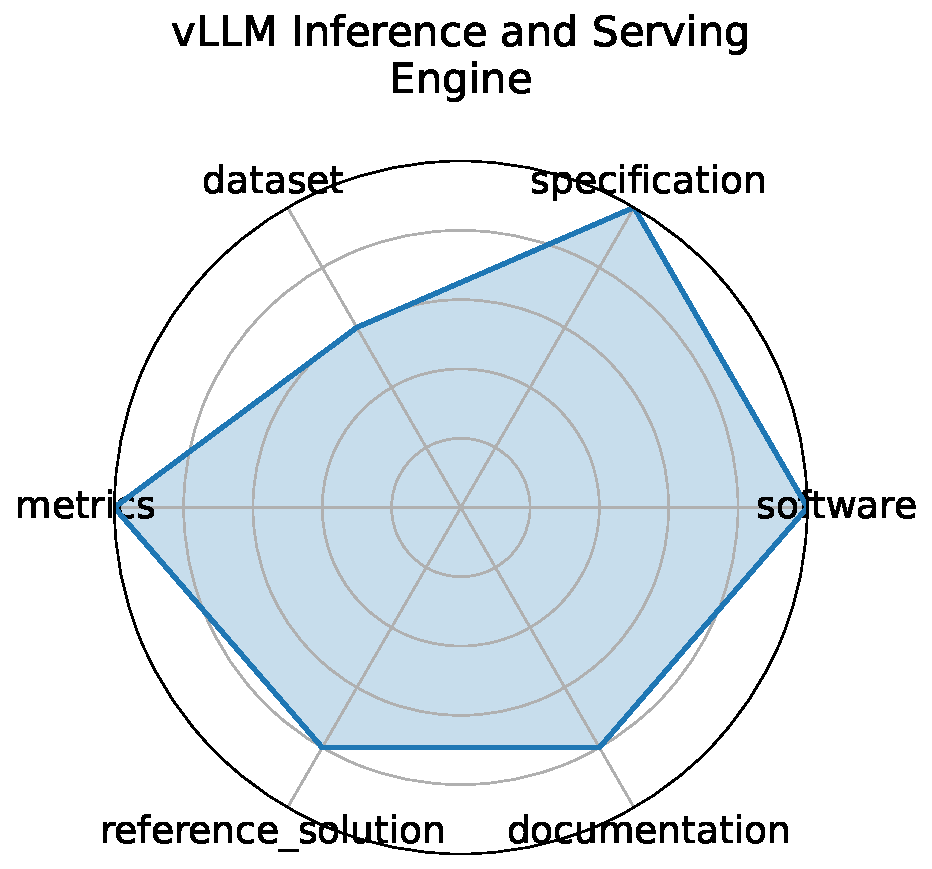
\includegraphics[width=0.2\textwidth]{vllm_inference_and_serving_engine_radar.pdf}
\end{description}
}}
\clearpage